\section{Определения}

\subsection{Машина Тьюринга.}

\textbf{Определение: } Формальное определние \textit{машины Тьюринга} -- это кортеж ($\Sigma, \Gamma, Q, q_1, q_a, q_r, \delta$), где
\begin{itemize}
    \item[$\Sigma$] -- конечное непустое множество -- входной алфавит, типично $\{0,1\}$.
    \item[$\Gamma$] -- конечное непустое множество, включающее в себя $\Sigma$, как подмножество, а также, по меньшей мере, еще пустой символ (бланк, пробел) -- ленточный алфавит.
    \item[$Q$] -- конечное множество, не пересекающееся с $\Gamma$ -- множество внутренних состояний.
    \item[$q_1$]$\in Q$ -- начальное состояние.
    \item[$q_a$]$\in Q$ -- принимающее состояние.
    \item[$q_r$]$\in Q$ -- отвергающее состояние.
    \item[$\delta$] -- функция перехода. $\delta: Q\times\Gamma \rightarrow Q\times\Gamma \times\{L, R, N\}$, где L -- перемещение влево, R -- вправо, N -- никуда.
\end{itemize}

Для задач с текстовым или числовым ответом вместо $q_r, q_a$ рассматривают одно $q_0$.

\textbf{Определение: } \textit{Конфигурация машины Тьюринга} -- данные о содержимом ленты, положении указателя и состоянии упавляющего блока.

Начальная конфигурация: на ленте написан вход, машина в состоянии $q$, указывает на первый символ входа. У каждой конфигурации есть однозначно опредляемая следующая. Если состояние завершающее, конфигурация уже не меняется. Иначе производится замена символа, состояния и положения головки.

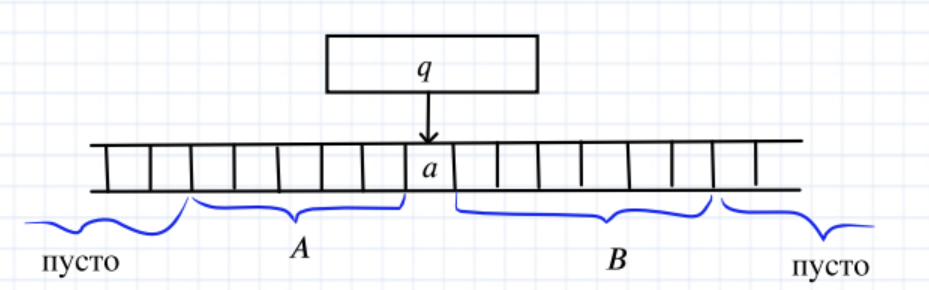
\includegraphics{images/3 (определения)_m31.PNG}

AqaB

\textit{Вычислением на машине Тьюринга} называется последовательность конфигураций, каждая из которых непосредственно следует из предыдущей по правилам этой машины.\\

\textbf{Пример смены конфигураций}

\begin{center}
    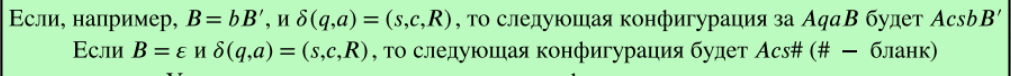
\includegraphics[width =17cm]{images/3 (определения)_mmm1.PNG}
\end{center}

q,s -- состояния

\subsection{Вычислимая функция.}

\textbf{Определение: } Функция $f: \{0,1\}^* \rightarrow \{0,1\}^*$ называется \textit{вычислимой}, если для некоторой машины Тьюринга выполнено:
\begin{itemize}
    \item[1] Если $f(x)$ определена, то существует вычисление, которое начинается с $q_{1}x$ и заканчивается $q_0f(x)$.
    \item[2] Если $f(x)$ не определена, то машина Тьюринга не остановится.
\end{itemize}

\textbf{Примеры}

\begin{center}
    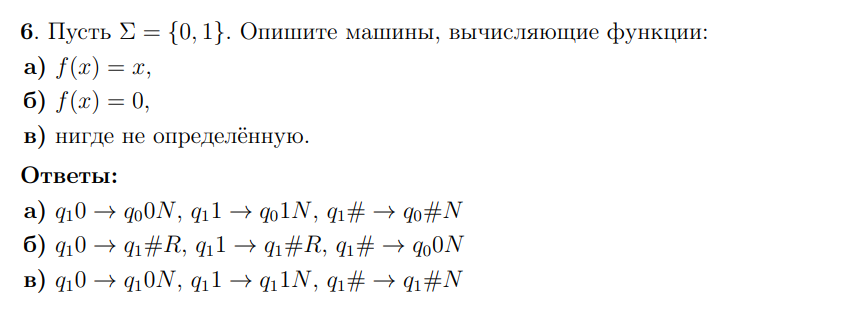
\includegraphics[width=15cm]{images/mt_1_def.png}
\end{center}

\subsection{Разрешимое множество.}

\textbf{Определение: } Множество $A \subset \{0,1\}^*$ называется \textit{разрешимым}, если для некоторой машины Тьюринга выполнено:
\begin{itemize}
    \item[1] Если $x \in A$, то существует вычисление на этой машине, которое начинается с $q_1x$ и заканчивается $q_a$.
    \item[2] Если $x \in \overline{A}$, то существует вычисление на этой машине, которое начинается с $q_1x$ и заканчивается $q_r$.
\end{itemize}

\subsection{Перечислимое множество.}

Будем рассматривать машину, у которой вместо завершающих состояний есть команды печати в поток вывода: печать 0, печать пробела. Результатом работы такой машины будет конечная или бесконечноая цепочка слов, разделенных пробелами.

\textbf{Определение: } Множество называется \textit{перечислимым}, если существует печатающая машина, такая что:
\begin{itemize}
    \item[] Если $x \in A$, то х встречается в потоке вывода.
    \item[] Если $x \not\in A$, то х не встречается в потоке вывода.
\end{itemize}

\textbf{Примеры}
\begin{itemize}
    \item [$\checkmark$] Пустое множество является перечислимым.
    \item [$\checkmark$] Область значений/Область определения любой вычислимой функции -- перечислимое множество.
    \item [$\times$] $\{n | U(n, x)$ определено при всех x$\}$ -- неперечислимо.
\end{itemize}

\subsection{Универсальная машина Тьюринга.}

\textbf{Определение: } \textit{Универсальная машина Тьюринга} -- это некоторая машина, которая получает на вход описание другой машины и вход для нее, а возвращает результат ее работы.
\[U(\langle M \rangle, x) = M(x).\]

\subsection{Универсальная вычислимая функция.}

\textbf{Определение: } Функция $u:\{0,1\}^* \times \{0,1\}^* \rightarrow \{0,1\}^*$ называется \textit{универсальной вычислимой функцией}, если:
\begin{itemize}
    \item[1] $u$ вычислима, как функция от двух аргументов.
    \item[2] Если $f:\{0,1\}^* \rightarrow \{0,1\}^* $ -- вычислимая функция одного аргумента, то $\exists p \forall x \ u(p,x) = f(x)$.
\end{itemize}

\subsection{Главная универсальная вычислимая функция.}

\textbf{Определение: } $U:\mathbb{N}\times\mathbb{N} \rightarrow \mathbb{N}$ -- \textit{главная универсальная вычислимая функция}, если
\begin{itemize}
    \item[1] $U$ вычислима.
    \item[2] $U$ универсальна, т.е. для любой вычислимой $f:\mathbb{N} \rightarrow \mathbb{N} $ найдется $p$ такое, что $\forall x f(x) = U(p,x)$ (говорят, что $p$ -- это номер функции $f$).
    \item[3] $U$ главная, т.е. для любой вычислимой $V: \mathbb{N}\times\mathbb{N} \rightarrow \mathbb{N}$ найдется всюду определенная вычислимая $s:\mathbb{N} \rightarrow \mathbb{N}$, такая что $\forall p \ \forall x \ V(p,x) = U(s(p),x)$.
\end{itemize}
Интуитивный смысл: $U$ -- универсальный компилятор, $V$ -- какой-то вычислимый. Первый аргумент $V$ -- \" \ программа\" \ , второй -- \" \ данные\" \ , $s$ -- \" \ автоматический траснлятор\" \ , переделывающие программу для $V$ в программу для $U$.

\subsection{$m$-сводимость.}

\textbf{Определение: } Говорят, что $A$ \textit{m-сводится} к $B$, если существует всюду определенная вычислимая функция $f:\mathbb{N} \rightarrow \mathbb{N}$, такая что $x \in A \lra f(x) \in B$. Обозначение: $A\leq_m B$.

\subsection{Арифметическая иерархия.}

\textbf{Определение: } Говорят, что множество $A $ принадлежит классу $\Sigma_n$, если существует такое разрешимое множество $R \in \mathbb{N}^{k+1}$, что
$$x \in A \lra \exists y_1 \ \forall y_2 \ \exists y_3 \ldots. \mathcal{Q} y_n [(x, y_1,\ldots,y_k) \in R].$$ 

Аналогично, говорят, что $A$ принадлежит классу $\Pi_n$, если существует такое разрешимое множество $R \in \mathbb{N}^{k+1}$, что
$$x \in A \lra \forall y_1 \ \exists y_2 \ \forall y_3 \ldots. \mathcal{Q} y_n [(x, y_1,\ldots,y_k) \in R].$$

Согласно этому определению, $\Sigma_0 = \Pi_0$ (классы $\Sigma_0$ и $\Pi_0$ совпадают с классом всех разрешимых множеств).

$\Sigma_1$ -- перечислимые, $\Pi_1$ -- коперечислимые

$\blacktriangle \ $S перечислимо $\lra$ для некоторого разрешимого R верно ($x \in S \lra \exists y \ (x,y) \in R$), Q коперечислимо $\lra$ для некоторого разрешимого R верно ($x \in S \lra \forall y \ (x,y) \in R$).

\textbf{Примеры}
\begin{itemize}
    \item[1] $T$ -- множество всюду определенных функций.
    
    $p \in T \lra \forall n \exists k (U(p,n)$ останавливается за $k$ шагов) -- разрешимое свойство $\Rightarrow T \in \Pi_2$.
    
    \item[2] $FD$ -- множество функций с конечной областью определения.
    
    $p \in FD \Leftrightarrow \exists N \forall n \ \forall k  (n > N \Rightarrow U(p,n)$ останавливается за k шагов) -- разрешимое свойство $\Rightarrow FD \in \Sigma_2$.
\end{itemize}

\subsection{$\lambda$-термы, $\alpha$-конверсии, $\beta$-редукции, нормальная форма.}

\textbf{Определение: } \textit{$\lambda$-терм} строится по индукции:
\begin{itemize}
    \item[1] Переменная является $\lambda$-термом.
    \item[2](Операция аппликации): Если M и N суть лямбда-термы, то (MN) - тоже лямбда-терм.
    
    Смысл: в функцию M вместо переменное подставляем N.
    \item[3](Операция $\lambda$-абстракции): Если M - терм, а x - переменная, то ($\lambda x.M$) - тоже терм.
    Смысл: выражение M теперь рассматривается как функция от х.
\end{itemize}

\textbf{Определение: } \textit{$\alpha$-конверсия} -- это замена связаной переменной. $\lambda x.M \rightarrow \lambda z.M(z/x)$

\textbf{Ограничение: не должно возникать конфликтов имен. Переменные из М не должны попадать под действие $\lambda$-квантора.}\\

\textbf{Пример}
\begin{itemize}
    \item [$\checkmark$] $\lambda x.xy \rightarrow \lambda z.zy$ -- так можно.
    \item [$\checkmark$] $\lambda x.xy(\lambda x.xy) \rightarrow \lambda z.zy(\lambda x.xy)$ -- и так можно.
    \item[$\times$] $\lambda x.xy \rightarrow \lambda y.yy$ -- а вот так нельзя.
    \item[$\times$] $\lambda x.x(\lambda y.xy) \rightarrow \lambda y.y(\lambda y.yy)$ -- и так тоже нельзя! Тут переменная, полученнная после замены, попала под воздействие уже имеющегося квантора.
\end{itemize}

\textbf{Определение: } \textit{$\beta$-редукция} -- это замена аргумента функции на какое-то значение. $(\lambda x.M)N \rightarrow M(N/x)$

\textbf{Ограничение: не должно возникать конфликтов имен. В N не должно быть переменных, по которым стоят $\lambda$-кванторы в М}\\

\textbf{Пример}
\begin{itemize}
    \item[$\checkmark$] sin x при x = 2 равен $\sin 2$.
    \item[$\times $] $(\lambda x.(x \lambda y.xy))y \rightarrow y\lambda y.yy$ -- так нельзя.
\end{itemize}

\textbf{Определение: } Говорят, что терм M находится в \textit{нормальной форме}, если к нему нельзя применить $\beta$-редукцию даже после нескольких $\alpha$-конверсий\\ Говорят, что N - нормальная форма M, если M = N и N находится в нормальной форме.

Не у всех термов есть нормальная форма.\\

\textbf{Пример}

$\Omega = (\lambda x.xx)(\lambda x.xx)$

\subsection{Нумералы Чёрча.}

\textbf{Определение: } 

Формально, число $k$ соответствует преобразованию функции $f$ в ее k-ую итерацию:

\begin{center}
    $\overline{0} = \lambda fx.x$
    
    $\overline{1} = \lambda fx.fx$
    
    $\overline{2} = \lambda fx.f(fx)$
    
    $\dots$
    
    $\overline{n} = \lambda fx. f(f\ldots f(fx))\ldots)$ -- $n$ раз $f$.
\end{center}

\subsection{Комбинатор неподвижной точки.}

\textbf{Определение: } \textit{Комбинатором} называется замкнутый $\lambda$-терм (без свободных переменных).

Говорят, что комбинатор $G$ представляет функцию $g: \mathbb{N}^k \rightarrow \mathbb{N}$, если для любых $n_1, \ldots, n_k$ выполнено:
\begin{center}
    $G\overline{n_1}\overline{n_2}\ldots\overline{n_k} = \overline{g(n_1,\ldots,n_k)}$. Если $g$ не определена, то у $G\overline{n_1}\overline{n_2}\ldots\overline{n_k}$ нет нормальной формы.
\end{center}
\textbf{Пример}
\begin{itemize}
    \item [1] Inc -- прибавление 1. Inc $\overline{n} = \overline{n} + 1$ : \\
    $Inc = \lambda nfx.f(nfx)$
    \item [2] Add -- сложение.  Add $\overline{n} \overline{m} = \overline{n + m}: \\
    Add = \lambda mn fx.mf(nfx)$
    \item[3] Mult -- умножение:\\
    $Mult = \lambda mn fx. m(nf)x$
     \item[4] Exp -- возведение в степень:\\
    $Exp = \lambda mn fx. nmfx$
\end{itemize}

\textbf{Определение: } $Y$ -- \textit{комбинатор неподвижной точки}, если для любого $F$ верно $YF = F(YF)$.

\textbf{Пример}
\begin{center}
    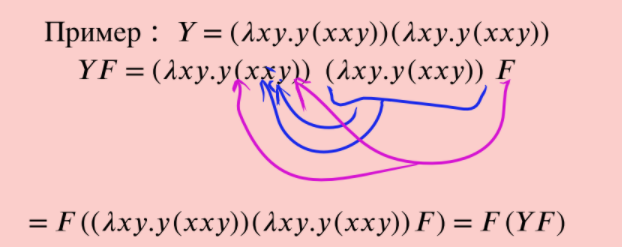
\includegraphics{images/3 (определения)_m32.PNG}
\end{center}
